%\VignetteIndexEntry{User manual}
\documentclass{article}\usepackage[]{graphicx}\usepackage[]{color}
%% maxwidth is the original width if it is less than linewidth
%% otherwise use linewidth (to make sure the graphics do not exceed the margin)
\makeatletter
\def\maxwidth{ %
  \ifdim\Gin@nat@width>\linewidth
    \linewidth
  \else
    \Gin@nat@width
  \fi
}
\makeatother

\definecolor{fgcolor}{rgb}{0.345, 0.345, 0.345}
\newcommand{\hlnum}[1]{\textcolor[rgb]{0.686,0.059,0.569}{#1}}%
\newcommand{\hlstr}[1]{\textcolor[rgb]{0.192,0.494,0.8}{#1}}%
\newcommand{\hlcom}[1]{\textcolor[rgb]{0.678,0.584,0.686}{\textit{#1}}}%
\newcommand{\hlopt}[1]{\textcolor[rgb]{0,0,0}{#1}}%
\newcommand{\hlstd}[1]{\textcolor[rgb]{0.345,0.345,0.345}{#1}}%
\newcommand{\hlkwa}[1]{\textcolor[rgb]{0.161,0.373,0.58}{\textbf{#1}}}%
\newcommand{\hlkwb}[1]{\textcolor[rgb]{0.69,0.353,0.396}{#1}}%
\newcommand{\hlkwc}[1]{\textcolor[rgb]{0.333,0.667,0.333}{#1}}%
\newcommand{\hlkwd}[1]{\textcolor[rgb]{0.737,0.353,0.396}{\textbf{#1}}}%

\usepackage{framed}
\makeatletter
\newenvironment{kframe}{%
 \def\at@end@of@kframe{}%
 \ifinner\ifhmode%
  \def\at@end@of@kframe{\end{minipage}}%
  \begin{minipage}{\columnwidth}%
 \fi\fi%
 \def\FrameCommand##1{\hskip\@totalleftmargin \hskip-\fboxsep
 \colorbox{shadecolor}{##1}\hskip-\fboxsep
     % There is no \\@totalrightmargin, so:
     \hskip-\linewidth \hskip-\@totalleftmargin \hskip\columnwidth}%
 \MakeFramed {\advance\hsize-\width
   \@totalleftmargin\z@ \linewidth\hsize
   \@setminipage}}%
 {\par\unskip\endMakeFramed%
 \at@end@of@kframe}
\makeatother

\definecolor{shadecolor}{rgb}{.97, .97, .97}
\definecolor{messagecolor}{rgb}{0, 0, 0}
\definecolor{warningcolor}{rgb}{1, 0, 1}
\definecolor{errorcolor}{rgb}{1, 0, 0}
\newenvironment{knitrout}{}{} % an empty environment to be redefined in TeX

\usepackage{alltt}
\usepackage{natbib}
\usepackage{fullpage}

\title{Using gemmR}

\author{Jeffrey S. Chrabaszcz and Joe W. Tidwell}
\IfFileExists{upquote.sty}{\usepackage{upquote}}{}
\begin{document}

\maketitle

\section*{Motivation}

In the social sciences, we often ask locational questions, such as:

\begin{itemize}
  \item Do people who train on certain computer tasks have \emph{higher} cognitive ability? \citep{tidwell2014counts}
  \item Are there \emph{more} murders per capita in more honor-focused cultures? \citep{dougherty2014deceptive}
  \item Does the native language \emph{change} acquisition of definite articles in a second language? \citep{chrabaszcz2014role}
\end{itemize}

These questions make no mention of the specific distance between relative groups and instead focus on the order of outcome magnitudes.
While the statistics applied to these questions are usually variants of the general linear model, there is no reason to impose the assumption of linearity on the reality underlying these tests.
One alternative is to apply the general monotone model (\texttt{GeMM}) as proposed by Dougherty \& Thomas, 2012 \citep{dougherty2012robust}.

\texttt{GeMM} uses a search and scale procedure to find the optimal relative weights for a set of predictors and scale these weights to minimize the order-constrained squared error.
This first, computationally-intensive step is accomplished by using a genetic algorithm to optimize some fit criterion (e.g., Kendall's $\tau$) between an observed outcome and a weighted set of predictors.
Use of $\tau$ in this case assures relative weights that maximally reflect the monotone relationship between the outcome and model predictions.
Other fit criteria penalize for complexity, but are based on transformations of $\tau$.
We then regress the original outcome onto the relative-weighted model predictions to compute an intercept and scaling factor that minimizes squared error conditioned on this ordinal constraint.

\section*{Fitting a \texttt{gemm} model}

We implement \texttt{GeMM} with the \texttt{gemmR} package, which uses \texttt{Rcpp} to speed up repeated calculation of Kendall's $\tau$ for use in the genetic search process.
As \texttt{GeMM} serves as a functional replacement for the linear model, a similar syntax is used to fit a \texttt{GeMM} model.

\begin{knitrout}
\definecolor{shadecolor}{rgb}{0.969, 0.969, 0.969}\color{fgcolor}\begin{kframe}
\begin{alltt}
\hlkwd{library}\hlstd{(gemmR)}
\hlkwd{data}\hlstd{(culture)}
\hlstd{mod} \hlkwb{<-} \hlkwd{gemm}\hlstd{(murder.rate} \hlopt{~} \hlstd{pasture} \hlopt{+} \hlstd{gini} \hlopt{+} \hlstd{gnp,} \hlkwc{data} \hlstd{= culture)}
\end{alltt}
\end{kframe}
\end{knitrout}

This produces a \texttt{gemm} object, which is modeled after the \texttt{lm} object.

\section*{Helper functions}

The \texttt{gemmR} package includes a number of S3 methods and a few novel functions to help extract information from \texttt{gemm} objects.

\subsection*{Summary}

\texttt{summary} displays some helpful information about the fitted \texttt{gemm} object.

\begin{knitrout}
\definecolor{shadecolor}{rgb}{0.969, 0.969, 0.969}\color{fgcolor}\begin{kframe}
\begin{alltt}
\hlkwd{summary}\hlstd{(mod)}
\end{alltt}
\begin{verbatim}
## Call:
## gemm.formula(formula = murder.rate ~ pasture + gini + gnp, data = culture)
## 
## Coefficients:
##      intercept pasture   gini        gnp
## [1,]    0.4286  0.2184 0.2500 -0.0001911
## [2,]    0.3280  0.2063 0.2524 -0.0001903
## [3,]    0.4391  0.2102 0.2499 -0.0001912
## [4,]    0.4263  0.2183 0.2501 -0.0001911
## 
## bic
## [1] -41.64 -41.64 -41.64 -41.64
\end{verbatim}
\end{kframe}
\end{knitrout}

\texttt{GeMM} is a stochastic process, so multiple replications are advisable to ensure stability of parameter estimates.
\texttt{gemm} runs four replications by default, all of which are displayed by descending value on the fit criterion.

Below the four chains are the corresponding values of the optimized fit criterion.
While all fit criteria are calculated and contained in the \texttt{gemm} object, only the criterion used for selection is displayed with \texttt{summary}.

\subsection*{Diagnostics}

Though no method exists for verifying that results of a random search process on empirical data, one quick way to check the suitability of a solution is to demonstrate convergent results across starting conditions.
A quick way to check genetic algorithm performance for a given dataset is to plot the best criterion value across generations and chains.

\begin{knitrout}
\definecolor{shadecolor}{rgb}{0.969, 0.969, 0.969}\color{fgcolor}\begin{kframe}
\begin{alltt}
\hlstd{check.mod} \hlkwb{<-} \hlkwd{gemm}\hlstd{(murder.rate} \hlopt{~} \hlstd{pasture} \hlopt{+} \hlstd{gini} \hlopt{+} \hlstd{gnp,} \hlkwc{data} \hlstd{= culture,} \hlkwc{check.convergence} \hlstd{=} \hlnum{TRUE}\hlstd{)}
\hlkwd{plot}\hlstd{(check.mod)}
\end{alltt}
\end{kframe}
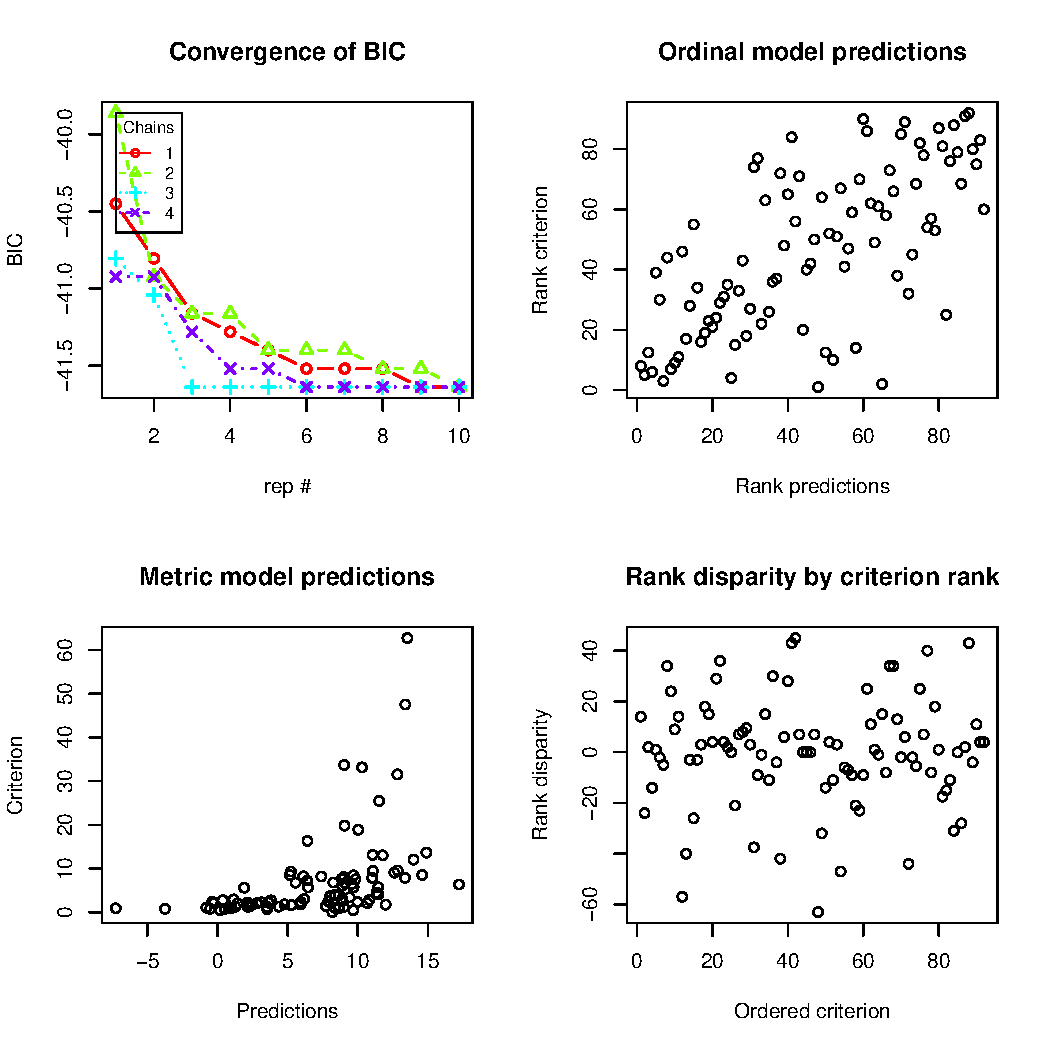
\includegraphics[width=\maxwidth]{figure/plotting} 

\end{knitrout}

\subsection*{Predict}

The \texttt{predict} function for \texttt{gemm} serves two roles.
The first is to generate model predictions based on the best chain of a given model.
\texttt{predict} will also generate the counts of concordances, disconcordances, outcome ties and predictor ties for a given model.

\begin{knitrout}
\definecolor{shadecolor}{rgb}{0.969, 0.969, 0.969}\color{fgcolor}\begin{kframe}
\begin{alltt}
\hlstd{yhat} \hlkwb{<-} \hlkwd{predict}\hlstd{(mod,} \hlkwc{tie.struct} \hlstd{=} \hlnum{TRUE}\hlstd{)}
\hlkwd{head}\hlstd{(yhat)}
\end{alltt}
\begin{verbatim}
##      [,1]
## 1  6.4641
## 2  7.7362
## 3 11.0760
## 4  8.8805
## 5  2.1789
## 6  0.5268
\end{verbatim}
\begin{alltt}
\hlkwd{attr}\hlstd{(yhat,} \hlstr{"tie.struct"}\hlstd{)}
\end{alltt}
\begin{verbatim}
##   correct incorrect cue.tie crit.tie
## 1    3118      1066       0        2
\end{verbatim}
\end{kframe}
\end{knitrout}

\subsection*{A note on information criteria in \texttt{gemmR}}

The information criteria calculated by \texttt{gemmR} are based on ordinal statistics and cannot be directly compared with likelihood-based criteria.
\texttt{gemmR} includes a number of methods so that traditional information criteria can be easily extracted for comparison with other models.

\begin{knitrout}
\definecolor{shadecolor}{rgb}{0.969, 0.969, 0.969}\color{fgcolor}\begin{kframe}
\begin{alltt}
\hlkwd{logLik}\hlstd{(mod)}
\end{alltt}
\begin{verbatim}
## 'log Lik.' -330.7 (df=1)
\end{verbatim}
\begin{alltt}
\hlkwd{AIC}\hlstd{(mod)}
\end{alltt}
\begin{verbatim}
## [1] 663.4
\end{verbatim}
\begin{alltt}
\hlkwd{BIC}\hlstd{(mod)}
\end{alltt}
\begin{verbatim}
## [1] 665.9
\end{verbatim}
\end{kframe}
\end{knitrout}

\bibliographystyle{plain}
\bibliography{gemm-vignette}

\end{document}
